\documentclass[UTF8, 12pt]{ctexart}

\usepackage{amsmath}

\usepackage{geometry}
\geometry{a4paper, scale = 0.9} % a4纸, 版心占页面长度的比例为0.9

\usepackage{enumitem} % itemize, 列表

\usepackage{graphicx}

\begin{document}

	\noindent
	频率响应的基本概念 :
	\begin{itemize}[leftmargin = 4em]
		\item 幅频特性 : 放大倍数随着频率变化的规律
		\item 相频特性 : 输出信号与输入信号的相位差随着频率变化的规律
		\item 通频带 : 幅频特性大于 $ \sqrt{0.5} $ 倍最大值的区域对应的频率
		\item 频率失真 : 放大电路对不同频率的增益不同, 相移不同, 导致的失真, 是线性失真; 原因 : 电抗性元件, 三极管的 $ \beta $ 与频率有关
		\item 波特图 : 横坐标(频率) : 对数刻度($ 10, 100, 1000, \cdots $); 纵坐标 : 幅频特性($ 20\lg|\dot{A}_{u}| $), 相频特性($ \phi $), 实际画图可以画折线
		\item 多级放大的波特图 : 各级相加即可
		\item 电路的截止频率, 取决于电容所在回路的时间常数
		\item 信号在下限频率/上限频率的时候, 增益下降3dB, 产生+45/-45的相移
	\end{itemize}

	波特图简单画法 :
	\begin{itemize}[leftmargin = 4em]
		\item 常数因子 : 幅频特性为常数, 相频特性为0
		\item $ j\omega $ 因子 : 幅频特性为+20dB/十倍频, 相频特性为+90
		\item $ \frac{1}{1+j\frac{\omega}{\omega_{p}}} $ 因子 : 幅频特性为从 $ \omega_{p} $ 开始的-20dB/十倍频, \\
			  相频特性为 $ (0, 0), (0.1\omega_{p}, 0), (10\omega_{p}, -90), (\infty, -90) $ 组成的折线段
		\item $ j\omega+\omega_{z} $ 因子 : 幅频特性为从 $ \omega_{z} $ 开始的+20dB/十倍频, \\
			  相频特性为 $ (0, 0), (0.1\omega_{z}, 0), (10\omega_{p}, 90), (\infty, 90) $ 组成的折线段
	\end{itemize}

	~

	\noindent
	简化混合 $ \pi $ 型等效电路 :

	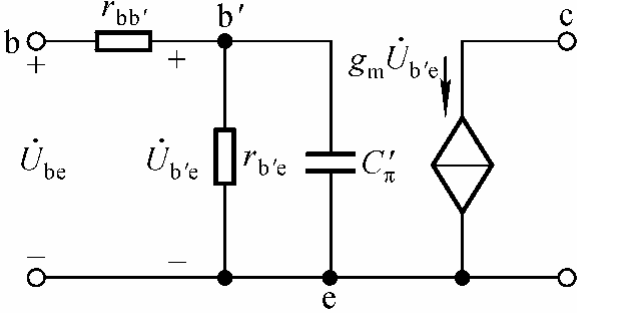
\includegraphics[scale = 0.4]{05/混合pi型等效电路电路图.png}

	~

	\noindent
	电流放大倍数 $ \beta $ 的频率响应 :

	$ \dot{\beta} = \frac{\beta_{0}}{1+j\omega r_{b'e}C'_{\pi}} = \frac{\beta_{0}}{1+j\frac{f}{f_{\beta}}} $, 其中 $ \beta_{0} $ 为中低频时的电流放大倍数, $ f_{\beta} = \frac{1}{2\pi r_{b'e}(C_{\pi}+C_{\mu})} $ 称作共射截止频率

	~

	\noindent 例子 :

	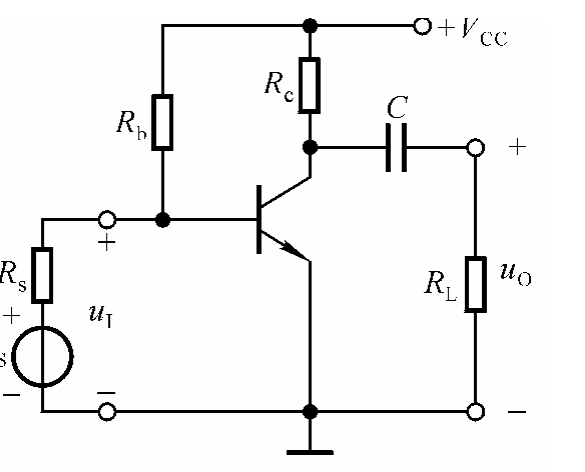
\includegraphics[scale = 0.4]{05/单管放大电路电路图.png}

	分析 :
	\begin{itemize}[leftmargin = 4em]
		\item 中频段(忽略所有电容) : $ \dot{A}_{usm} = -\frac{R_{i}}{R_{i}+R_{s}}\frac{r_{b'e}}{r_{bb'}+r_{b'e}}g_{m}(R_{C} \parallel R_{L}), \varphi = -180 $
		\item 低频段(忽略 $ C'_{\pi} $) : $ \dot{A}_{usL} = \dot{A}_{usm}\frac{jf/f_{L}}{1+jf/f_{L}}, f_{L} = \frac{1}{(R_{C}+R_{L})C}, \varphi = -180+90-\arctan(f/f_{L}) $
		\item 高频段(忽略 $ C $) : $ \dot{A}_{usH} = \dot{A}_{usm}\frac{1}{1+j\omega RC'_{\pi}}, f_{H} = \frac{1}{2\pi RC'_{\pi}}, \varphi = -180-arctan(f/f_{H}) $
	\end{itemize}

	增益-带宽积(GBP) = $ |\dot{A}_{usm}(f_{H}-f_{L})| $, 提高增益时带宽会变窄; 多级放大电路会增加增益, 但是通频带会变窄.

\end{document}